\documentclass{beamer}
\mode<presentation>
\usepackage{amsmath}
\usepackage{amssymb}
\usepackage{algorithmic}
%\usepackage{advdate}
\usepackage{adjustbox}
\usepackage{subcaption}
\usepackage{enumitem}
\usepackage{multicol}
\usepackage{mathtools}
\usepackage{listings}
\usepackage{url}
\def\UrlBreaks{\do\/\do-}
\usetheme{Boadilla}
\usecolortheme{lily}
\setbeamertemplate{footline}
{
  \leavevmode%
  \hbox{%
  \begin{beamercolorbox}[wd=\paperwidth,ht=2.25ex,dp=1ex,right]{author in head/foot}%
    \insertframenumber{} / \inserttotalframenumber\hspace*{2ex} 
  \end{beamercolorbox}}%
  \vskip0pt%
}
\setbeamertemplate{navigation symbols}{}

\providecommand{\nCr}[2]{\,^{#1}C_{#2}} % nCr
\providecommand{\nPr}[2]{\,^{#1}P_{#2}} % nPr
\providecommand{\mbf}{\mathbf}
\providecommand{\pr}[1]{\ensuremath{\Pr\left(#1\right)}}
\providecommand{\qfunc}[1]{\ensuremath{Q\left(#1\right)}}
\providecommand{\sbrak}[1]{\ensuremath{{}\left[#1\right]}}
\providecommand{\lsbrak}[1]{\ensuremath{{}\left[#1\right.}}
\providecommand{\rsbrak}[1]{\ensuremath{{}\left.#1\right]}}
\providecommand{\brak}[1]{\ensuremath{\left(#1\right)}}
\providecommand{\lbrak}[1]{\ensuremath{\left(#1\right.}}
\providecommand{\rbrak}[1]{\ensuremath{\left.#1\right)}}
\providecommand{\cbrak}[1]{\ensuremath{\left\{#1\right\}}}
\providecommand{\lcbrak}[1]{\ensuremath{\left\{#1\right.}}
\providecommand{\rcbrak}[1]{\ensuremath{\left.#1\right\}}}
\theoremstyle{remark}
\newtheorem{rem}{Remark}
\newcommand{\sgn}{\mathop{\mathrm{sgn}}}
\providecommand{\abs}[1]{\left\vert#1\right\vert}
\providecommand{\res}[1]{\Res\displaylimits_{#1}} 
\providecommand{\norm}[1]{\lVert#1\rVert}
\providecommand{\mtx}[1]{\mathbf{#1}}
\providecommand{\mean}[1]{E\left[ #1 \right]}
\providecommand{\fourier}{\overset{\mathcal{F}}{ \rightleftharpoons}}
%\providecommand{\hilbert}{\overset{\mathcal{H}}{ \rightleftharpoons}}
\providecommand{\system}{\overset{\mathcal{H}}{ \longleftrightarrow}}
	%\newcommand{\solution}[2]{\textbf{Solution:}{#1}}
%\newcommand{\solution}{\noindent \textbf{Solution: }}
\providecommand{\dec}[2]{\ensuremath{\overset{#1}{\underset{#2}{\gtrless}}}}
\newcommand{\myvec}[1]{\ensuremath{\begin{pmatrix}#1\end{pmatrix}}}
\let\vec\mathbf

\lstset{
%language=C,
frame=single, 
% breaklines=true,
columns=fullflexible
}

\numberwithin{equation}{section}

\title{Find the Curve of the Differential Equation Through the Given Point}
\author{S A Aravind Eswar - EE24BTECH11053}

\date{\today} 
\begin{document}

\begin{frame}
\titlepage
\end{frame}

\section*{Outline}
\begin{frame}
\tableofcontents
\end{frame}

\section{Problem}
\begin{frame}
\frametitle{Problem Statement}
    Solve the differntial equation,
    \begin{align}
        \frac{dy}{dx} + 2y = \sin{x}
    \end{align}
    with inital conditions $x=0$ and $y=0$
\end{frame}

%\subsection{Literature}
\section{Solution}

\subsection{Laplace Transform in brief}
\begin{frame}
    \frametitle{Laplace Transform in brief}
    Let, $f(t)$ be a piece-wise continuous function, then Laplace transform of the $f(t)$ is denoted as $\mathcal{L}\cbrak{f(t)}$ and is defined as,
    \begin{align}
        \mathcal{L}\cbrak{f(t)} = \int_{0}^{\infty} e^{-s\,t}f(t)\,dt = F(s)
    \end{align}
    It is a linear operator, meaning it follows superposition and homogeneity.

    It has an inverse operation denoted as $\mathcal{L}^{-1}\cbrak{F(s)} = f(t)$.

    A property of Laplace transform we will use for solving the problem,
    \begin{align}
        \mathcal{L}\cbrak{f^{(n)}} = s^n F(s) - s^{n-1} f(0) - s^{n-2} f^\prime(0) - \dots - f^{(n-1)}(0) 
    \end{align}
\end{frame}

\subsection{Theoretical Solution}
\begin{frame}[allowframebreaks]
    \frametitle{Theoretical Solution}
    \begin{align}
        y^\prime + 2y = \sin{x}\\
    \end{align}
    Applying Laplace Transform,
    \begin{align}
        \mathcal{L}\cbrak{y^\prime} + 2\mathcal{L}\cbrak{y} &= \mathcal{L}\cbrak{\sin{x}}\\
        \cbrak{sY-y(0)} + 2 \cbrak{Y} &= \frac{1}{s^2 + 1}
    \end{align}

    Simplifying,

    \begin{align}
        Y &= \frac{1}{(s+1)(s^2+1)}\\
        Y &= \brak{\frac{1}{s^2 + 1}- \frac{s}{s^2+1} + \frac{1}{s+2}}\frac{1}{5}
    \end{align}

    Applying inverse transform,
    \begin{align}
        y = \frac{2\sin{x}-\cos{x}+e^{-2x}}{5}
    \end{align}
\end{frame}

\subsection{Fininte Difference Method}
\begin{frame}
\frametitle{Finite Difference Method}
    Difference equation can be written as,
    \begin{align}
        \frac{dy}{dx} \approx \frac{y_{n+1}-y_n}{h}\\
        y_{n+1} = y_n + \frac{dy}{dx}\, h
    \end{align}
    Substituting,
    \begin{align}
        \frac{dy}{dx} = \sin{x} - 2y
    \end{align}
    we get,
    \begin{align}
        y_{n+1} = y_n + \brak{\sin{x_n} - 2y_n}\,h
    \end{align}
\end{frame}

\subsection{Algorithm}
\begin{frame}
    \frametitle{Algorithm}
        \begin{algorithmic}
            \STATE \text{Initial condition, } $x_0 \gets 0$\\
            % \STATE \text{End value of domain, } $x_2 \gets 5$\\
            % \STATE $x \gets$ linspace($x_1$, $x_2$, $resolution$)
            % \STATE $y \gets$ array of size($resolution$)
            \STATE $y_0 \gets 0$
            \STATE \text{Number of iterations, } $iterations \gets 20$\\
            \STATE \text{Step size, } $h = 0.25$
            \FOR{$i$ in range(1, $iterations$)}
                \STATE $\displaystyle y_{i} = y_{i-1} + \brak{\sin{x_{i-1}} - 2y_{i-1}}\, h$
                \STATE $x_i \gets x_{i-1} + h$
            \ENDFOR
            \STATE plot($x, y$)
        \end{algorithmic}
\end{frame}

\subsection{Plotting the curve}
\begin{frame}
\frametitle{Plotting the curve}
\begin{figure}[h]
    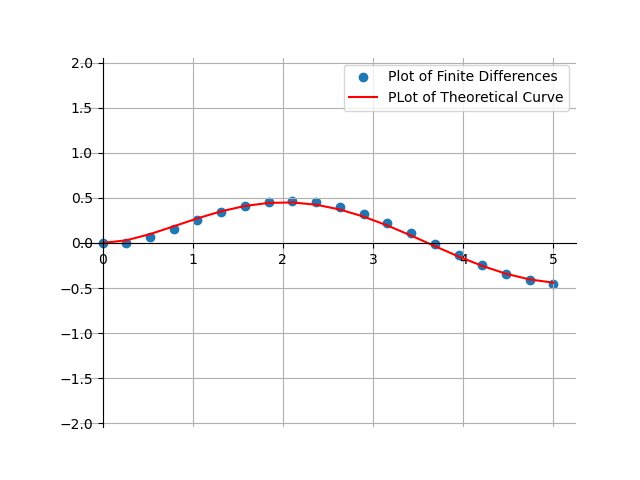
\includegraphics[scale=0.6]{../figs/fig1_.png}
\centering
\end{figure}
\end{frame}
%\section{Plot}
% \subsection{Integration}
% \begin{frame}
% \frametitle{Integration}

% Calculating $A_1$ and $A_2$,
% \begin{align}
% A_1 = \int_0^4 \frac{x^2}{4} dx = \frac{16}{3}\\
% A_2 = \int_0^{2\sqrt{2}} \frac{x^2}{4} dx = \frac{4\sqrt{2}}{3}
% \end{align}

% Final area,

% \begin{align}
% A = \brak{\int_0^4 4 dx - A_1} - \brak{\int_0^{2\sqrt{2}}2 dx - A_2} = \frac{32-8\sqrt{2}}{3}
% \end{align}

% \end{frame}
% \subsection{Code}
% \begin{frame}[fragile, allowframebreaks]
%     \frametitle{Code}
%     Code for generating the points using C:
%     \lstset{
%         language = C,
%         basicstyle=\ttfamily\small,
%         keywordstyle=\color{blue},
%         stringstyle=\color{green},
%         commentstyle=\color{gray},
%         tabsize=4
%     }
%     % \lstinputlisting{./codes/points.c}
    
%     Code for plotting the graph of the curve and area using Python:
%     \lstset{
%         language=Python,
%         basicstyle=\ttfamily\small,
%         keywordstyle=\color{blue},
%         stringstyle=\color{green},
%         commentstyle=\color{gray},
%         tabsize=4
%     }
%     % \lstinputlisting{./codes/plot.py}

%     The codes in: 
%     {\footnotesize
%         \begin{lstlisting}
% https://github.com/me-coder-1204/EE1030/blob/main/Assignment5/codes/plot.py
% https://github.com/me-coder-1204/EE1030/blob/main/Assignment5/codes/points.c
%         \end{lstlisting}
%     }
% \end{frame}
\end{document}
